% This is samplepaper.tex, a sample chapter demonstrating the
% LLNCS macro package for Springer Computer Science proceedings;
% Version 2.20 of 2017/10/04
%
\documentclass[oribibl]{llncs}
%
\usepackage{graphicx}
\usepackage{enumitem}
\usepackage{bm}
\usepackage{amsfonts}
\usepackage{mathtools}
\usepackage{blindtext}
\usepackage[capitalise]{cleveref}
\usepackage[british]{babel}
\usepackage{geometry}
\usepackage{graphicx,psfrag,epsf}
\usepackage{enumerate}
\usepackage{enumitem}
\usepackage{amssymb}
\usepackage{amsmath}
\usepackage{longtable}
\usepackage{bigints}
%\usepackage{siunitx}
\usepackage{soul}
\usepackage{tikz}
\usepackage{color}
\usepackage{easyReview} % for \comment, \alert, etc.

\newcommand{\x}{\boldsymbol{X}}
\renewcommand{\b}{\hat{\beta}}
\newcommand{\reals}{\mathbb{R}}
\newcommand{\normal}{\mathcal{N}}
\newcommand{\lexp}{\underline{\text{E}}}
\newcommand{\uexp}{\overline{\text{E}}}


\begin{document}

\title{A Robust Bayesian Approach for Causal Inference Problems
%\thanks{}
}
%
\author{Tathagata Basu\inst{1}\orcidID{0000-0002-6851-154X} \and
Matthias C.~M.~Troffaes\inst{2}\orcidID{0000-0002-1294-600X} \and
Jochen Einbeck\inst{2,3}\orcidID{0000-0002-9457-2020}}
%
\authorrunning{Basu et al.}
%
\institute{Civil and Environmental Engineering, University of Strathclyde, UK \
Department of Mathematical Sciences, Durham University, UK \
Durham Research Methods Centre, UK}
%
\maketitle              
%
\begin{abstract}
Causal inference using observational data is an important aspect in
many fields such as epidemiology, social science, economics, etc. In
particular, our goal is to find the treatment effect on the subjects
along with the causal links between the variables and the outcome.
However, estimation for such problems are extremely
difficult as the treatment effects may vary from subject
to subject and modelling the underlying heterogeneity explicitly makes the
problem practically unsolvable. Another issue we often face is the
dimensionality of the problem and we need to find a subset of
explanatory variables to understand the treatment effect.
However, currently variable selection methods tend to maximise the
predictive performance of the underlying model. This can be problematic
in the case of limited information. As in many cases, the consequence of
mistreatment can be harmful. So, in this paper, we considering for a
robust Bayesian analysis which accounts for abstention in selecting
an explanatory variable in the high dimensional regression model.
To achieve that, we consider a set of spike and slab priors
through prior elicitation to obtain set of posteriors for
both the treatment and outcome model. We are specifically interested
in the sensitivity of the treatment effect in the high dimensional causal
inference as well as the identifying the confounder variables by means
of variable selection. However, confounder selection can be deceptive
in this setting. Especially, when a predictor is strongly associated
with either the treatment or the outcome. This will increase the posterior
expectation of the selection probability and might abstain from rejecting
this variable as a confounder. To avoid that we apply a post-hoc selection scheme
which successfully remove negligible non-zero effects from the model
attaining a smaller set of confounders as well as seperate sets of variables
which are only related to treatment or outcome model. Finally, we illustrate
our method to show it's applicability in real life scenarios.

\keywords{high dimensional data \and variable selection \and Bayesian analysis \and imprecise probability.}
\end{abstract}


\section{Introduction}\label{sec:intro}

In causal inference, we are interested in estimating the causal
effect of independent variables on a dependent variable. Ideally,
randomised trials are the most efficient way to perform this task.
However, this is not very practical for several reasons; ethical 
concerns, design cost, population size, to name a few. This
leaves us with observational studies which are usually obtained
by means collecting data though surveys or record keeping. But this
can be problematic in the presence of confounders. That is when
the variables are associated with both the treatment and the outcome.
In such cases, we need to be extra cautious as otherwise it will
lead to unwanted bias in the treatment effect estimator \cite{rosenbaum83}.
Several works have been done in order to tackle the presence of
confounder variables. One such work in the topic was 
by Robins \cite{Robins1986ANA} where the author used  a graphical
approach for the identification of the causal parameters.
Rosenbaum and Robin \cite{rosenbaum1985} suggested the use of a link model to estimate
the propensity scores for all individuals. Later on several other
methods have been proposed based on propensity score matching.
A brief review on such methods can be found in \cite{winship99, stuart10}.

Bayesian approaches in causal effect estimation is a popular
strategy in the field and one of the earlier works on this can be
found in \cite{rubin1978}. Lately, with the rise of high dimensional 
data, Bayesian methodologies have become
more appealing. Crainiceanu \text{et al.~}\cite{Crainiceanu2008} proposed a bi-level 
Bayesian model averaging based method for estimating the causal 
effect. Wang \text{et al.~}\cite{wang2015} suggested BAC (or, Bayesian adjustment for
confounding) where they use an informative prior obtained from
the treatment model and apply them on the outcome model for
estimating causal effect. Several other methods were also
proposed to tackle confounders from the point of view of Bayesian
variable selection such as: \cite{Zigler2014}, \cite{Hahn2018} etc.

In this paper we take inspiration from the approach of Koch \text{et al.~}\cite{koch2020}, where
they proposed a bi-level spike and slab prior for causal effect 
estimation. They considered a data-driven adaptive approach to
propose their prior which reduce the variance of the causal estimate. 
In our approach, we perform a 
sensitivity analysis based approach where instead of using a single prior, 
we consider a set of priors \cite{BERGER1990303}. This is particularly 
interesting as in many cases, causal effect estimation can be performed 
through a meta analysis and hence robust Bayesian analysis \cite{raices_cruz22} 
can be beneficial under severe uncertainty. Moreover, for some problems 
we have to rely on very limited data to perform our Bayesian analysis and 
inference may not be reliable in presence of hetaroskedasticity within
the data. Instead, we use expert opinion and elicit a set of priors 
based on empirical evidence. 
This also allows us to construct the problem of confounder identification 
in a framework where abstention has a relatively positive gain ie.~
the cost of further tests/data collection is cheaper than
mistreating a subject. To propose our 
framework, we consider a set of continuous spike and slab priors 
\cite{ishwaran2005} for confounder identification and construct a Bayesian 
group LASSO \cite{xu2015} type problem. To perform the prior sensitivity 
analyses, we consider a set of beta priors on the covariate selection 
probability of the spike and slab priors. We use the posteriors of these
covariate selection probability for identifying the confounders. Finally, 
we consider a post-hoc coefficient adjustment method \cite{hahn2015}
to recover sparse estimates associated with either the outcome or the
treatment model. 

The rest of the paper is organised as follows. In \cref{sec:causal}
we give a formal description of causal estimation problem in the
context of linear regression. \cref{sec:bayes} is focused on the
Bayesian analysis of causal inference problems, followed by the
motivation of a robust Bayesian analysis along with our proposed decision 
theoretic framework for confounder (variable) selection. In \cref{sec:sim}, 
we provide our result of simulation studies under different scenarios 
and to show the applicability in real life problems. Finally, 
we discuss our findings and conclude this paper in \cref{sec:conc}.

\section{Causal Estimation}\label{sec:causal}

Let an observational study give us the outcomes $Y=(Y_1$, \dots, $Y_n)$ along with 
corresponding treatment indicators $T=(T_1$, \dots, $T_n)$. Then the
treatment 
effect in the population is given by the expectation of the difference
in outcome between the treatment and controls. 
\begin{align}
	\delta = \mathbb{E}(Y\mid T =1) - E(Y\mid T=0).
\end{align}
Similarly, individual causal
effect of the treatment $T_i$ on outcome $Y_i$ is given by:
\begin{align}
	\delta_i \coloneqq (Y_i\mid T_i=1) - (Y_i\mid T_i=0).
\end{align}
That is, the difference between the outcome when $i$-th subject receives
the treatment and when $i$-th subject remain as a control. 

In theory, both of these quantities exist.
However, we can not observe $(Y_i\mid T_i=1)$ and $(Y_i\mid T_i=0)$
simultaneously for the $i$-th individual. Instead, we can estimate
average causal effect of the treatment $T$ by calculating the averaged
outcome of all the subjects those received the treatment and
all the subjects those remained as control.
\begin{align}
	\hat{\delta} \coloneqq 
	\frac{\sum_{i=1}^n Y_i\cdot\mathbb{I}(T_i=1) - 
		\sum_{i=1}^n Y_i\cdot\mathbb{I}(T_i=0)}{n}.
\end{align}
However, this relies on an important assumption that the treatment effect
on the $i$-th subject given that they received the treatment is
equal to the treatment effect when they remain as the control
\cite{winship99}.

\subsection{Regression Model}
Regression methods are widely used in causal effect estimation. The
main idea behind these regression methods is to remove the
correlation between the treatment indicator and the error term
\cite{winship99,HECKMAN1985}. To do so, we rely on $p$ different observed quantities
or predictors denoted by $X\coloneqq$ $[X_1$, \dots, $X_n]^T$. Now, let
$\beta \coloneqq (\beta_1$, \dots, $\beta_p)$ denotes the vector of regression
coefficients. Then we can define a linear model for the outcome
so that
\begin{equation}
	Y_i = \beta_{T} T_i + \beta_0 + X_i\beta + \epsilon_i
\end{equation}
where $\epsilon_i\sim \mathcal{N}(0, \sigma^2)$. Clearly, when
the underlying true outcome model is linear with respect to the treatment,
\begin{equation}
	\delta = \mathbb{E}(Y\mid T =1) - E(Y\mid T=0) = \beta_{T}.
\end{equation}
In the presence of confounders we also need to consider the
association between the treatment indicators and the predictors.
In literature, authors often suggested the use of a probit link function to 
construct the regression model. This way, we can
specify the conditional probability that subject $i$ receives the treatment through a linear model. 
That is, for another vector of regression coefficients 
$\gamma\coloneqq(\gamma_1, \cdots, \gamma_p)$ we define
\begin{align}
	P(T_i=1\mid X_i) \coloneqq \Phi(\gamma_0+X_i\gamma)
\end{align}
where $\Phi(\cdot)$ denotes the cumulative distribution function
of a standard normal distribution. To incorporate this probit
link function, we define intermediate latent variables as suggested
by \cite{albert93}
\begin{equation}
	T_i^* = \gamma_0 + X_i\gamma +u_i
\end{equation}
where, $u_i\sim\mathcal{N}(0,1)$. Therefore, $T_i=1$ if $\Phi(\gamma_0+X_i\gamma)
>1/2$ and hence $T_i^*>0$. Similarly, $T_i=0$ if $T_i^*\le0$. 

Now, to construct the joint likelihood function, we define an appended
output vector $W\coloneqq(Y, T^*)^T$ and corresponding $2n\times(2p+3)$ dimensional design matrix
\begin{align}
	Z &=
	\begin{bmatrix}
		X_O & 0 \\
		0 & X_T
	\end{bmatrix},
\end{align}
where, $X_O = [T, 1_n, X]$ and $X_T = [1_n, X]$. Then, considering the assumption of
Gaussian error terms, we have the following likelihood distribution
\begin{align}
	W\mid Z, \alpha, \beta, \gamma, \sigma^2 \sim\normal\left(Z\nu, \Sigma\right)\label{eq:like:group},
\end{align}
where $\nu = (\beta_T, \beta_0, \beta, \gamma_0, \gamma)^T$ and
\begin{align}
	\Sigma &=
	\begin{bmatrix}
		\sigma^2{I}_n & 0 \\
		0 & {I}_n
	\end{bmatrix}.
\end{align}


\section{Bayesian Causal Estimation}\label{sec:bayes}

The likelihood formation given by \cref{eq:like:group} gives us
a foundation for Bayesian group LASSO 
\cite{xu2015} type model and look into the posterior selection
probability associated with the $j$-th predictor. There are several
ways to construct spike and slab priors which achieve 
variable selection. In our case, we consider a continuous type
\cite{ishwaran2005} prior for faster posterior
computation.


\subsection{Hierarchical model}

Let, $\pi_j$ denote the prior probability that the $j$-th
predictor is associated to either the outcome or the 
treatment. That is, 
\begin{equation}
	\pi_j = P\left((\beta_j,\gamma_j)\not=(0,0)\right).
\end{equation}
Then we can define the following hierarchical model for spike and 
slab group LASSO so that,
for $1\le j\le p$,
\begin{align}
	(\beta_j,\gamma_j)^T \mid \pi_{j}, \sigma^2 &\sim 
	\pi_{j}\normal\left( \begin{bmatrix}
		0 \\
		0
	\end{bmatrix}, 
	\tau_1^2\begin{bmatrix}
		\sigma^2 & 0 \\
		0 & 1
	\end{bmatrix}\right)
	+ (1-\pi_{j}) \normal\left(\begin{bmatrix}
		0 \\
		0
	\end{bmatrix}, 
	\tau_0^2\begin{bmatrix}
		\sigma^2 & 0 \\
		0 & 1
	\end{bmatrix}\right)\\
	\beta_T, \beta_0\mid \sigma^2 &\sim \normal\left(0, \sigma^2\right)\\
	\gamma_0 &\sim \normal(0,1)\\
	\sigma^2&\sim \text{InvGamma}(a, b)\\
	\pi_{j} &\sim\text{Beta}\left(sq_j, s(1-q_j)\right).
\end{align}
In the hierarchical model, we fix sufficiently small $\tau^2_0$
$(1\gg\tau_0^2>0)$ so that  $(\beta_j, \gamma_j) = (0,0)$ has its probability mass 
concentrated around zero. Therefore, this represents the spike component of our prior specification. 
For the slab component, we consider $\tau_1^2$ to be large so that $\tau_1^2\ge 1$. This allows the prior for $(\beta_j, \gamma_j)\not=(0,0)$ to be flat. 
We illustrate the components of a bivariate spike and slab prior in 
\cref{fig:ssbl} (with fixed $\sigma=1$). We generate the spike component 
with $\tau_0=0.001$ and the slab component with $\tau_1=5$.

\begin{figure}[h]
	\begin{center}
		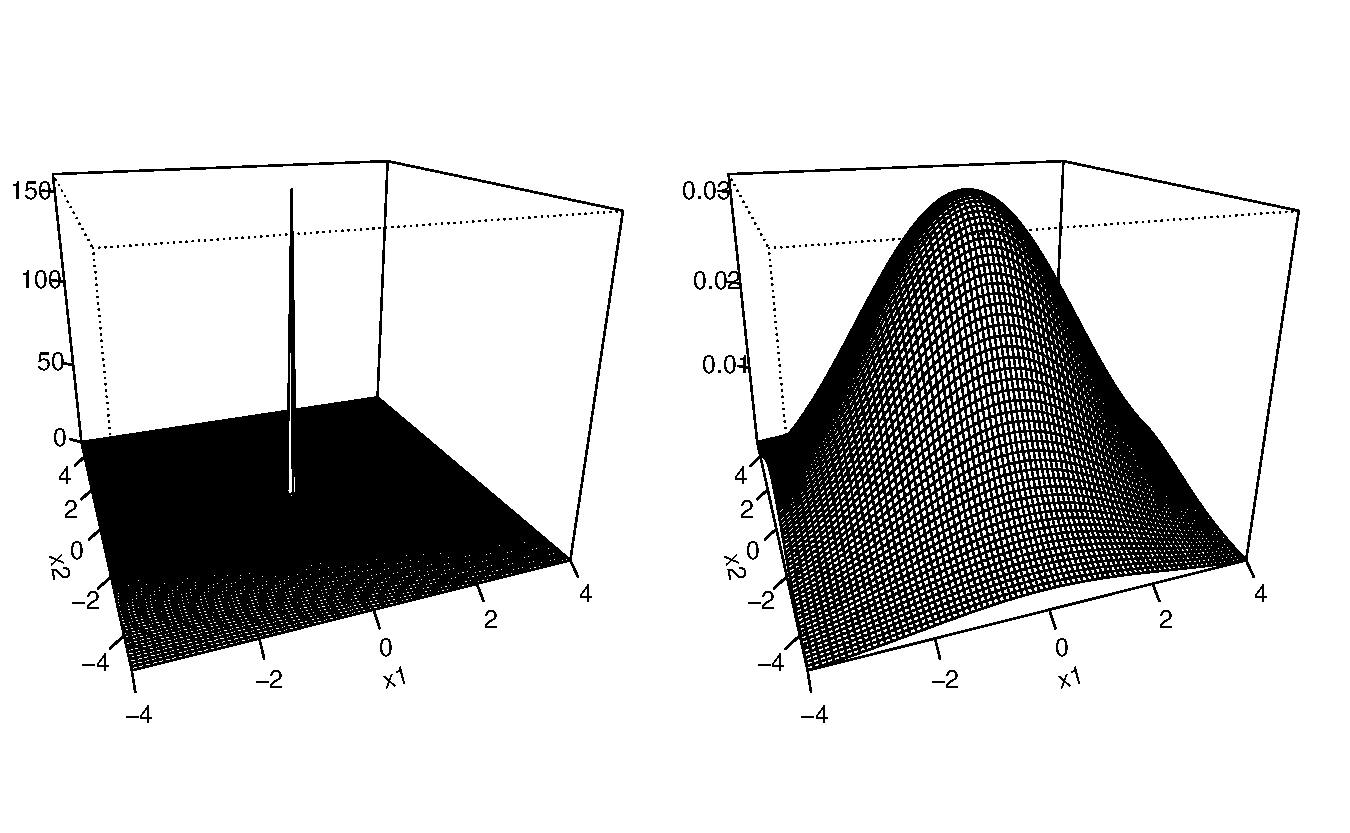
\includegraphics[width = 0.95\linewidth]{spike_slab_bi.pdf}
	\end{center}
	\caption{Spike and slab components of a bi-variate distribution for $\tau_0 = 0.001$, $\tau_1$ = 5 and $\sigma=1$.}
	\label{fig:ssbl}
\end{figure}

For the variance term $\sigma^2$, a natural choice of prior is inverse-Gamma 
because of conjugacy properties with Gaussian distribution. To
ensure that the prior is flat, we consider $1\ge a, b >0$.
As defined earlier, $\pi_j$ is used as the selection probability
of the $j$-th predictor in either of the models and we use a beta prior to specify 
these selection probabilities where  $q_j$ represents our prior expectation of the selection probability ($\pi_j$) and `$s$' acts as 
a concentration parameter.
For the intercept term of the outcome model and the causal effect, 
we want to use a Gaussian distribution that matches the scale of the noise term.
Therefore, we consider $\beta_0. \beta_T\sim \normal(0,\sigma^2)$. 
Similarly, for the intercept term in the treatment model, we consider 
$\gamma_0\sim \normal(0,1)$ as we use a probit link function. 

In \cref{fig:regress}, we show a probabilistic graphical representation
of our hierarchical model. In the figure, grey circular nodes represent the
prior hyper-parameters which will be used for sensitivity analysis
of the model. The transparent circular nodes are used to denote
the modelling parameters which are our quantities of interest. 
The observed quantities are denoted with transparent rectangular
nodes. We also use a grey rectangular node to denote the intermediate
latent variable $T^*$. We use directed edges to denote the
relationship between different nodes. However, we use a dashed
edge between $X$ and $T$ as they are related through the latent
variable $T^*$. 

\begin{figure}
	\centering
	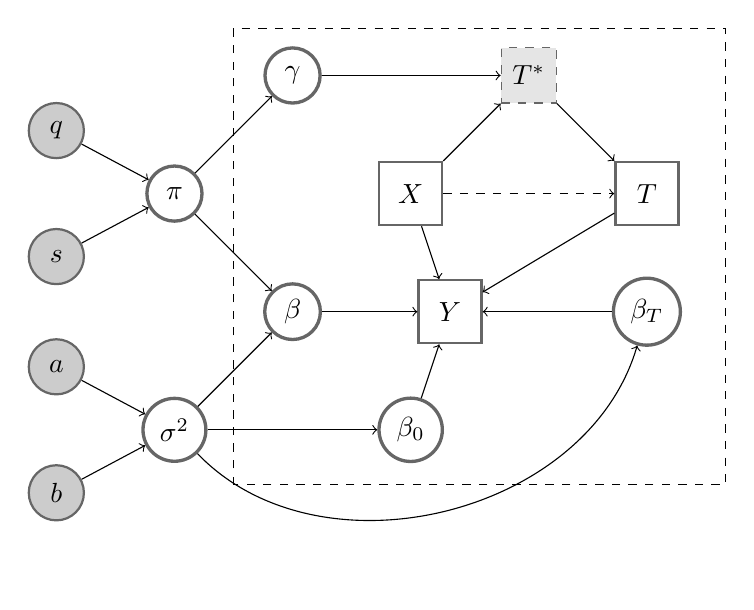
\begin{tikzpicture}[params/.style={circle, draw=black!60, very thick, minimum size=7mm},
		hyper/.style={circle, draw=black!60, fill=black!20, thick, minimum size=7mm},
		post/.style={circle, draw=black!60, fill=green!20, thick, minimum size=7mm},
		latent/.style={rectangle, draw=black!60, fill=black!10, dashed, minimum size=7mm},
		data/.style={rectangle, draw=black!60, thick, minimum size=8mm}]
		\node[params] (1) at (0,0) {$\pi$};
		\node[data] (2) at (3,0) {$X$};
		\node[data] (3) at (6,0) {$T$};
		\node[params] (4) at (1.5,1.5) {$\gamma$};
		\node[latent] (5) at (4.5,1.5) {$T^*$};
		\node[params] (6) at (1.5,-1.5) {$\beta$};
		\node[data] (7) at (3.5,-1.5) {$Y$};
		\node[params] (8) at (0,-3) {$\sigma^2$};
		\node[params] (9) at (3,-3) {$\beta_0$};
		\node[params] (10) at (6,-1.5) {$\beta_T$};
		\node[hyper] (11) at (-1.5,-.8) {$s$};
		\node[hyper] (12) at (-1.5,.8) {$q$};
		\node[hyper] (13) at (-1.5,-2.2) {$a$};
		\node[hyper] (14) at (-1.5,-3.8) {$b$};
		\draw[black, dashed] (0.75,-3.7) rectangle (7,2.1);
		
		\path (1) edge[->]  (6);
		\path (1) edge[->]  (4);
		\path (8) edge[->]  (6);
		\path (6) edge[->]  (7);
		\path (2) edge[->]  (7);
		\path (2) edge[->]  (5);
		\path (5) edge[<-] (4);
		\path (5) edge[->] (3);
		\path (3) edge[->]  (7);
		\path (9) edge[->]  (7);
		\path (10) edge[->]  (7);
		\path (2) edge[dashed][->] (3);
		\path (8) edge[bend right = 60][->]  (10);
		\path (8) edge[->]  (9);
		\path (11) edge[->]  (1);
		\path (12) edge[->]  (1);
		\path (13) edge[->]  (8);
		\path (14) edge[->]  (8);
		
	\end{tikzpicture}
	\caption{Probabilistic graphical representation for causal inference with Bayesian hierarchical model.}
	\label{fig:regress}
\end{figure}

\subsection{Robust Bayesian Analysis}
We perform our
robust Bayesian analysis on $q\coloneqq(q_1$, \dots, $q_p)\in\mathcal{P}$, where
\begin{equation}
	\mathcal{P} \coloneqq \mathcal{P}_1\times\cdots\times\mathcal{P}_p\subseteq \left(0, 1\right)^{p}.
\end{equation}

\subsection{Variable selection and coefficient adjustment}
For the co-variate selection, we look into the posterior expectation of $\pi_j$. 
We consider the $j$-th predictor to be removed from both the
treatment and outcome model, if
\begin{align}
	\lexp (\pi_j\mid W)\coloneqq \inf_{q_j\in \mathcal{P}_j} \text{E}(\pi_j\mid W) > 1/2.
\end{align}

For the rest of the variables, some of them will be present
in the model as confounders and some will only be associated with
either the treatment. Let $\mathcal{S}$ denote the set of
predictors such that,
\begin{equation}
	\mathcal{S}\coloneqq
	\left\{j : \lexp(\pi_j\mid W) < 1/2\right\}.
\end{equation}
That is the set that contains all the variables which are not
removed from both treatment and outcome model. Now, for
each fixed value of $q$,
let $\hat{\beta}_{\mathcal{S}}(q_{\mathcal{S}})$ be the posterior means of the regression coefficients of the outcome model with respect to
the predictors that belong to $\mathcal{S}$. Similarly,
$\hat{\gamma}_{\mathcal{S}}(q_{\mathcal{S}})$ be the posterior means of the regression
coefficients for the treatment effects. Since, we use a continuous type
selection prior, these regression coefficients are non-zero in nature.
Therefore, to adjust the sparsity, we apply the 
``decoupled shrinkage and selection'' method proposed by \cite{hahn2015}. To do so, we solve the following adaptive LASSO-type \cite{Zou2006}
problems

\begin{align}
	\hat{\beta}^*_{\mathcal{S}}(q) &= 
	\arg\min_{\beta_{\mathcal{S}}} \frac{1}{n}\|X_{\mathcal{S}}\hat{\beta}_{\mathcal{S}}(q)
	- X_{\mathcal{S}} \beta_{\mathcal{S}}\|_2^2 + \lambda\sum_{j\in\mathcal{S}} 
	\frac{|\beta_j|}{|\hat{\beta}_j(q_j)|}
\end{align}
and
\begin{align}
	\hat{\gamma}^*_{\mathcal{S}}(q) &= 
	\arg\min_{\gamma_{\mathcal{S}}} \frac{1}{n}\|X_{\mathcal{S}}\hat{\gamma}_{\mathcal{S}}(q)
	- X_{\mathcal{S}} \gamma_{\mathcal{S}}\|_2^2 + \lambda\sum_{j\in\mathcal{S}} 
	\frac{|\gamma_j|}{|\hat{\gamma}_j(q_j)|}
\end{align}
where $q_{j}\in \mathcal{P}_{j}$ for all $j\in\mathcal{S}$.

\iftrue
\subsection{Causal effect adjustment} The DSS method explained
above give us adjusted coefficient estimates for the treatment
and outcome model. However, as result the causal effect estimate
remains the same and modelling with such adjusted sparse effect 
will contribute to the prediction error. Therefore, we need to 
adjust the causal effect estimate as well. We do that in three steps
similar to double residual regression procedure as suggested by
\cite{robinson1988}.

First we compute the predicted values of $Y$ with respect to
the adjusted regression coefficients so that,
\begin{equation}
	\hat{Y}(q) 
	= \hat{\beta}_0(q) + X_{\mathcal{S}}\hat{\beta}^*_{\mathcal{S}}(q)
\end{equation}
and the values of $T$ with respect to the adjusted
regression coefficients so that
\begin{equation}
	\hat{T}(q) 
	= \Phi\left(\hat{\gamma}_0(q) + X_{\mathcal{S}}\hat{\gamma}^*_{\mathcal{S}}(q)\right).
\end{equation}
Then we estimate the adjusted causal effect using the following linear
model
\begin{equation}
	\left(Y-\hat{Y}(q)\right) = \left(T - \hat{T}(q)\right)\beta_{T} + \epsilon^*_i.
\end{equation}
That is 
\begin{equation}
	\beta_{T}^* = \left(\left(T - \hat{T}(q)\right)^T\left(T - \hat{T}(q)\right)\right)^{-1}\left(T - \hat{T}(q)\right)^T\left(Y-\hat{Y}(q)\right)
\end{equation}

\fi


\section{Simulation Studies}\label{sec:sim}


\section{Conclusion}\label{sec:conc}

\bibliographystyle{splncs04}
\bibliography{basu22}

\end{document}
